%%%%%%%%%%%%%%%%%%%%%%%%%%%%%%%%%%%%%%%%%%%%%%%%%%%%%%%%%%%%%%%%%%%%%%%%%%%%%%%%
%2345678901234567890123456789012345678901234567890123456789012345678901234567890
%        1         2         3         4         5         6         7         8

\documentclass[letterpaper, 10 pt, conference]{ieeeconf}  % Comment this line out
                                                          % if you need a4paper
                                                          % use the \thanks command
%\documentclass[a4paper, 10pt, conference]{ieeeconf}      % Use this line for a4
                                                          % paper

\IEEEoverridecommandlockouts                              % This command is only
                                                          % needed if you want to
                                                          % use the \thanks command
\overrideIEEEmargins
% See the \addtolength command later in the file to balance the column lengths
% on the last page of the document



% The following packages can be found on http:\\www.ctan.org
\usepackage{graphics} % for pdf, bitmapped graphics files
\usepackage{epsfig} % for postscript graphics files
%\usepackage{mathptmx} % assumes new font selection scheme installed
%\usepackage{times} % assumes new font selection scheme installed
\usepackage{amsmath} % assumes amsmath package installed
\usepackage{amssymb}  % assumes amsmath package installed
\usepackage{hyperref}
\usepackage{verbatim}
\usepackage{caption}
\usepackage{clrscode3e}

\title{\LARGE \bf
Modelling the behavior of a soft material-actuator
}

\author{%Aslan Miriyev, Sam Cohen, Neil Chen%Huibert Kwakernaak$^{1}$ and Pradeep Misra$^{2}$% <-this % stops a space
\begin{tabular}{ c c c }
\renewcommand{\arraystretch}{1}
	Aslan Miriyev & Sam Cohen & Neil Chen \\
    \href{aslan.miriyev@columbia.edu}{aslan.miriyev@columbia.edu} & \href{slc2206@columbia.edu}{slc2206@columbia.edu} & \href{neil.chen@columbia.edu}{neil.chen@columbia.edu}
\end{tabular}
}
\begin{document}
\renewcommand{\arraystretch}{1.2}

\maketitle
\thispagestyle{empty}
\pagestyle{empty}

%%%%%%%%%%%%%%%%%%%%%%%%%%%%%%%%%%%%%%%%%%%%%%%%%%%%%%%%%%%%%%%%%%%%%%%%%%%%%%%%
\begin{abstract}
%Inspired by natural muscle, a key challenge in soft robotics is to develop self-contained electrically driven soft actuators with high strain density. Various characteristics of existing technologies, such as the high voltages required to trigger electroactive polymers ( > 1KV), low strain ( < 10%) of shape memory alloys and the need for external compressors and pressure-regulating components for hydraulic or pneumatic fluidicelastomer actuators, limit their practicality for untethered applications. Here we show a single self-contained soft robust composite material that combines the elastic properties of a polymeric matrix and the extreme volume change accompanying liquid–vapor transition. The material combines a high strain (up to 900%) and correspondingly high stress (up to 1.3 MPa) with low density (0.84 g cm−3). Along with its extremely low cost (about 3 cent per gram), simplicity of fabrication and environment-friendliness, these properties could enable new kinds of electrically driven entirely soft robots.
Self-contained electrically-driven soft actuators with high strain density, low cost, simple fabrication methods, and low current draw represent a key challenge in soft robotics. We present several methods for predictive analysis of the behavior of such an actuator, with a focus on time-series analysis of actuator load and wear.
\end{abstract}


%%%%%%%%%%%%%%%%%%%%%%%%%%%%%%%%%%%%%%%%%%%%%%%%%%%%%%%%%%%%%%%%%%%%%%%%%%%%%%%%
\section{INTRODUCTION}
A soft, robust, self-contained composite material-actuator exhibiting high actuation stress along with very high actuation strain resolves many of the issues confronted by traditional soft actuation solutions (FEAs, PAMs, DEAs, etc.). The complex electrical, chemical, and physical behavior of these actuators, however, presents multiple steady-state and transient response controls problems.

Here we approach one of these problems: we attempt to evaluate the load characteristic, and in turn the wear, of a single soft material-actuator sample over time.

We evaluate the performance of three separate approaches to modelling the behavior of this soft material-actuator:
\begin{enumerate}
	\item Function approximation of actuator load cycle behavior via deep learning.
  \item Regression analysis on derived features of actuator load cycle characteristic.
  \item Fourier analysis/time-series autoregression methods.
\end{enumerate}

Ultimately we find that more input features and/or samples are necessary to usefully model the behavior of such an actuator.

%This template, modified in MS Word 2003 and saved as ÒWord 97-2003 \& 6.0/95 Ð RTFÓ for the PC, provides authors with most of the formatting specifications needed for preparing electronic versions of their papers. All standard paper components have been specified for three reasons: (1) ease of use when formatting individual papers, (2) automatic compliance to electronic requirements that facilitate the concurrent or later production of electronic products, and (3) conformity of style throughout a conference proceedings. Margins, column widths, line spacing, and type styles are built-in; examples of the type styles are provided throughout this document and are identified in italic type, within parentheses, following the example. Some components, such as multi-leveled equations, graphics, and tables are not prescribed, although the various table text styles are provided. The formatter will need to create these components, incorporating the applicable criteria that follow.

\section{DATA}

\subsection{Experimental Setup}
The experimental setup and data generation process consists of a new (or \href{https://www.cambridge.org/core/journals/mrs-communications/article/rejuvenation-of-soft-materialactuator/0D5EA2D555F28C616AB00B773DDFF313}{rejuvenated}) actuator sample enclosed in an Instron load cell. The actuator is sufficiently constrained such that it can neither extend nor contract.

During measurement, a cycle begins whenever \verb|Load| reaches $0N$. At the peak of a cycle, a \verb|Load| threshold of roughly $135N$ has been reached, and current is no longer supplied to the actuator. Thus cycle \verb|Load| minima and maxima remain roughly fixed between cycles. This behavior is visible in \textbf{Figure 1}.%\textbf{Figure \ref{CyclesOverlaid}}.

\subsection{Dataset}

The dataset (\verb|raw_cycles.csv|, which can be downloaded \href{https://github.com/Columbia-Creative-Machines-Lab/muscle-prediction}{here}) consists of $2$ features and $170,103$ time-series samples measured at $0.100s$ intervals. Please preview the dataset online, or refer to \textbf{Table I} for more information. %\textbf{Table \ref{Dataset}}, for more information.

The data represents $47$ actuation \textit{cycles}. A \textit{cycle} consists of a \textit{heating} phase and a cooling phase. During \textit{heating}, the actuator exerts positive force, and thus \verb|Load| is convex increasing with time. During \textit{cooling}, the actuator gradually exerts less force, and thus \verb|Load| is convex decreasing with time. 

\begin{table}[h] % h for here, not the top of the document
  \centering
  \begin{tabular}{ c | c c }
      Feature & Unit & Format \\
      \hline
      \verb|Time| & seconds & 3 decimal places \\
      \verb|Load| & Newtons & 5 decimal places
  \end{tabular}
  \label{Dataset}
  \caption{Unit and format of features in input dataset.}
\end{table}

\label{CyclesOverlaid}
\begin{figure}[h]
	\centering
	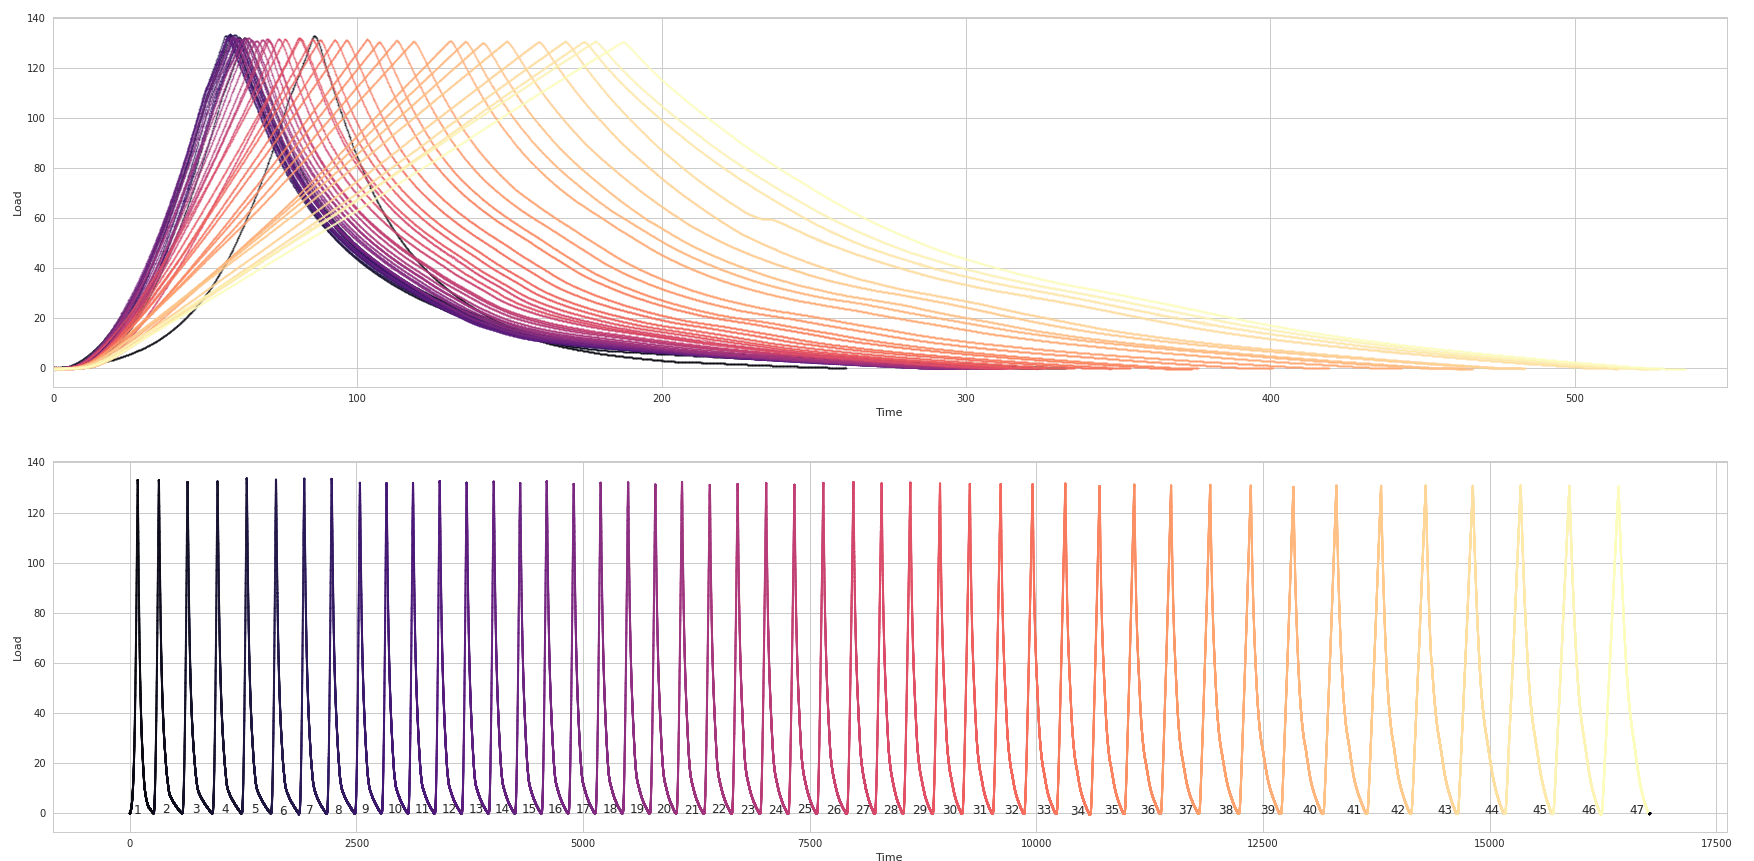
\includegraphics[width=0.5\textwidth]{assets/cyclesoverlaid.png}
    \caption{Heating-cooling cycles over time.}
\end{figure}

Specified in this manner, the dataset consists of $47$ complete cycles. Note that the local maximum and local minimum \verb|Load| values of each cycle are roughly equal.

\subsection{Exploratory Data Analysis}

We begin by plotting and quantifying certain characteristics of the dataset.

\label{heatingcooling}
\begin{figure}[h]
	\centering
  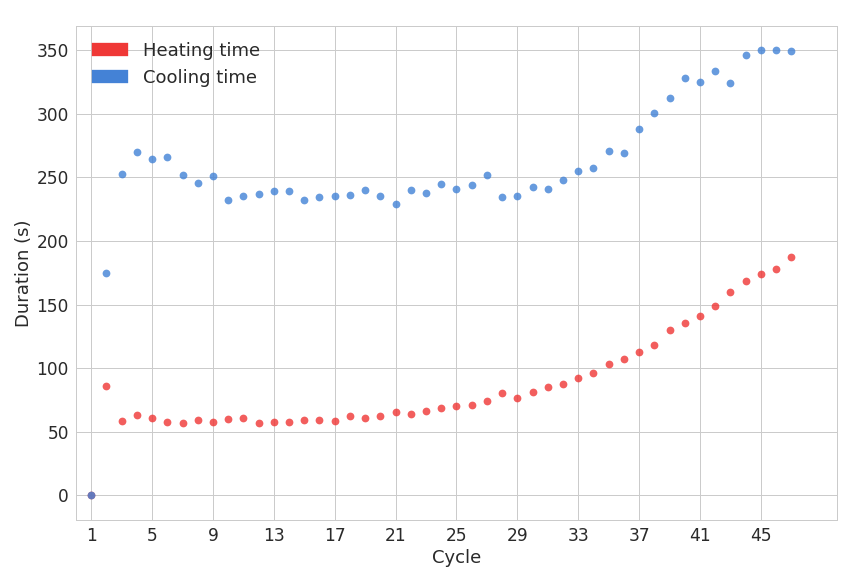
\includegraphics[width=0.5\textwidth]{assets/heatingcooling.png}
    \caption{Heating and cooling duration as a function of cycle number.}
\end{figure}

\label{tailperiod}
\begin{figure}[h]
	\centering
  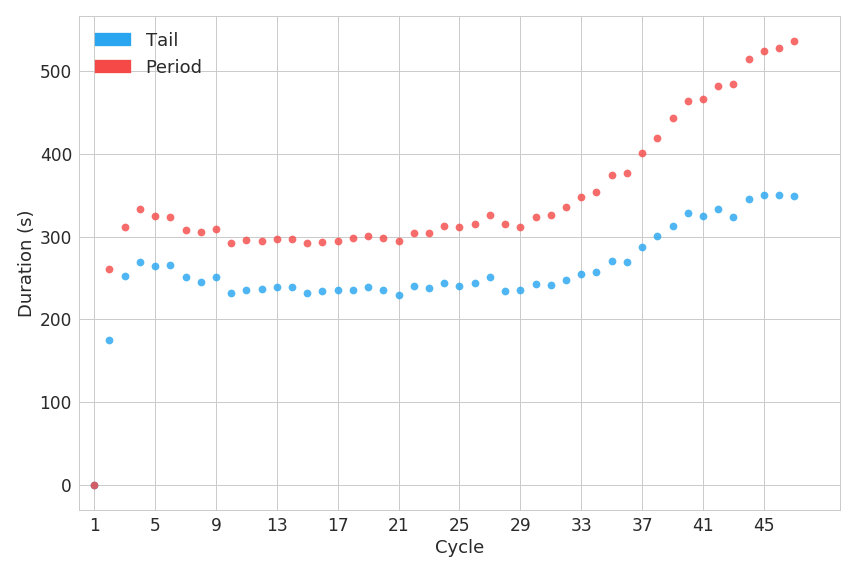
\includegraphics[width=0.5\textwidth]{assets/tailperiod.png}
    \caption{Tail (time elapsed while \texttt{Load} $\leq \big{(} 0.1 \times $\texttt{Max Load}$\big{)}$ and period duration as a function of cycle number.}
\end{figure}

\label{belly}
\begin{figure}[h]
	\centering
  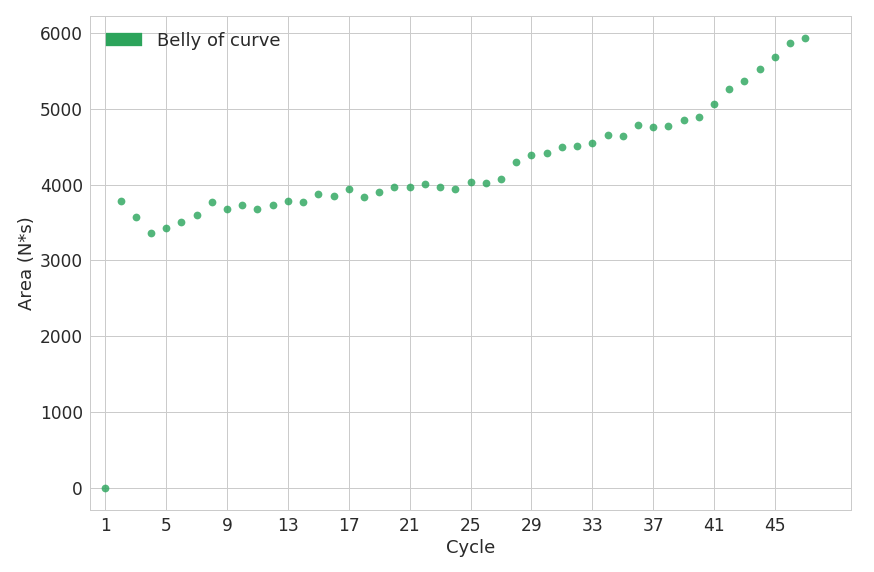
\includegraphics[width=0.5\textwidth]{assets/belly.png}
    \caption{Belly-of-cooling-curve area as a function of cycle number.}
\end{figure}

\label{area}
\begin{figure}[h]
	\centering
  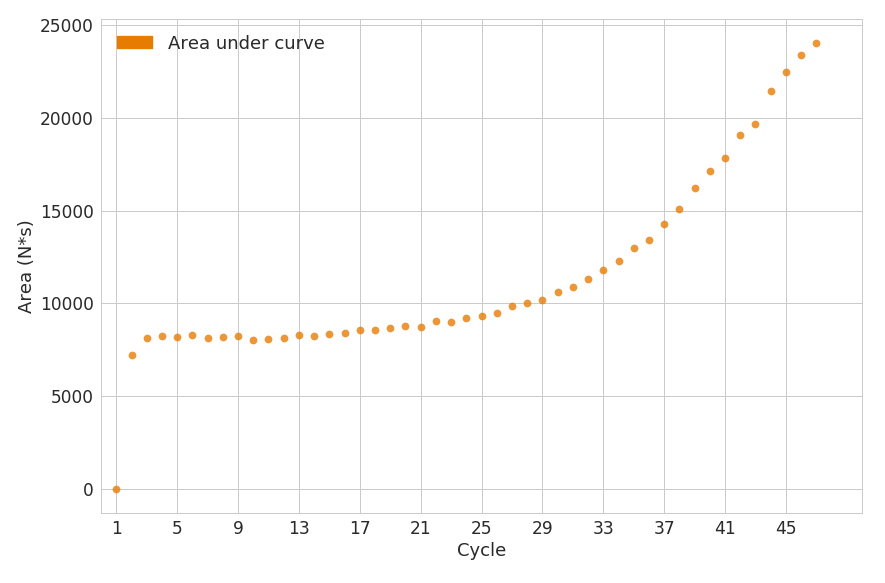
\includegraphics[width=0.5\textwidth]{assets/area.png}
    \caption{Area under \texttt{Load} function as a function of cycle number.}
\end{figure}

%\begin{enumerate}
%\itemsep0em 
%\item Cycle period over cycle number:  \textbf{Figure \ref{PeriodGrowth}}
%\item Cycle heating time over cycle number: \textbf{Figure \ref{HeatingDurations}}
%\item Cycle cooling time over cycle number: \textbf{Figure \ref{CoolingDurations}}
%
%\end{enumerate}


%\label{PeriodGrowth}
%\begin{figure}[h]
%	\centering
%	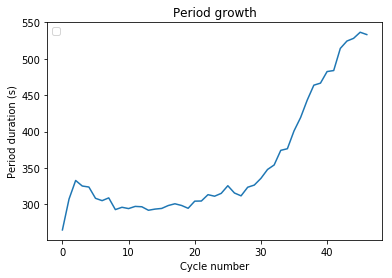
\includegraphics[width=0.5\textwidth]{assets/period_growth.png}
%    \caption{\textbf{Figure \ref{PeriodGrowth}.} Period growth as a function of cycle number.}
%\end{figure}
%
%\label{HeatingDurations}
%\begin{figure}[h]
%	\centering
%	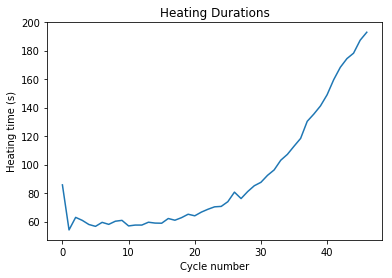
\includegraphics[width=0.5\textwidth]{assets/heating_durations.png}
%    \caption{\textbf{Figure \ref{HeatingDurations}.} Heating duration as a function of cycle number.}
%\end{figure}
%
%\label{CoolingDurations}
%\begin{figure}[h]
%	\centering
%	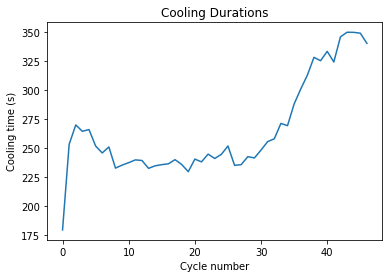
\includegraphics[width=0.5\textwidth]{assets/cooling_durations.png}
%    \caption{\textbf{Figure \ref{CoolingDurations}.} Cooling duration as a function of cycle number.}
%\end{figure}

We find that the average cycle heating and cooling times are $91.29$ seconds and $265.32$ seconds, respectively. We also note that cooling and heating durations appear to grow exponentially over the number of cycles. This trend is likely due to a variety of physical phenomena occurring within the actuator, such as gradual ethanol escape and internal heat build up.

\section{DERIVED FEATURES}

\subsection{Motivation}

We attempt to inject expert knowledge about the actuator system's behavior by constructing $11$ derived features. These features encode approximately constant maximum/minimum-\verb|Load| behavior, $n^\text{th}$-order moments of each cycle, cycle index, and more. Each feature is manually computed over the entire dataset; derived features are excluded from validation/testing sets.

\subsection{Computation}

\textbf{Table II} enumerates all derived features.

%\clearpage
\begin{table}[h]
  \centering
  \begin{tabular}{ c | c }
    \textbf{Feature} & \textbf{Meaning} \\
    \hline
    Time & Absolute time since $0.00s$ \\
    Load & Absolute load from $0N$ \\
    Min & One-hot encoding of local minima \\
    Max & One-hot encoding of local maxima \\
    Cycle & Index of cycle from $0$ \\
    Area & Area under cycle curve, calculated as $\int_{t_{min}}^{t_{max}}$ \verb|Load| $dt_i$ \\
    Heating & Time elapsed while heating, calculated as $t_{max} - t_{min}$ \\
    Cooling & Time elapsed while cooling, calculated as $t_{end} - t_{max}$ \\
    HCprop & Proportion $\frac{\texttt{Heating}}{\texttt{Cooling}}$ of heating time to cooling time \\
    Period & Period of cycle, equivalent to \verb|Heating| $+$ \verb|Cooling| \\
    Tail & Time elapsed while $\verb|Load| \leq \big{(}0.1 \times \verb|Max Load|\big{)}$ \\
    Belly & \begin{tabular}{c} Multiple integral between \verb|Cooling| curve and \\ line tangent to both \verb|Max Load| and \verb|Load|$_{t_{end}}$\end{tabular} \\
    Kurt & Kurtosis of curve (fourth standardized moment) \\
    Skew & Skewness of curve
  \end{tabular}
  \label{derived}
  \caption{All derived features and calculations involved.}
\end{table}
%%%%%%%%%%%%%%%%%%%%%%%%%%%%%%%%%

\section{Regression analysis}
We use the following approach to generate models and evaluate their performance on derived feature prediction:
\begin{enumerate}
  \item Generate time-series cross-validation training-validation splits, delimiting data by each cycle.
  \item Perform grid-search on regression parameters to identify models which best predict derived features
\end{enumerate}

We then develop a regression model from these derived features:
\begin{enumerate}
  \item Split cycles into four piecewise curves, as enumerated in \textit{IV.A}.
  \item Perform grid-search on regression parameters, minimizing loss (per piecewise curve) between predicted \verb|Load| and ground truth \verb|Load| as a function of \verb|Time|. 
\end{enumerate}

\subsection{Piecewise cycle splitting}\label{ssec:Piecewise}
We split curves into continuous piecewise sections using two simple methods: fixed boundaries and $K$-means clustering.

\subsubsection{Fixed boundaries}
We delimit curves at four points. Let $t_0 = 0$ denote the time at which a cycle begins; $t_{max} =$ the time at which a cycle reaches its maximum \verb|Load|; and $t_f$ denote the time at which a cycle finishes, such that $t_f =$ the \verb|Period| of a cycle. Then:

\begin{align*}
  t_1 &= \frac{t_{max} - t_0}{2} \\
  t_2 &= t_{max} \\
  t_3 &= \frac{t_f - t_{max}}{2}
\end{align*}

and we regress separately on the following subsections of a cycle's \verb|Period|. Let $c_i=$ the set of observations in the $i^{\text{th}}$ cycle of the dataset $X$. Then we define the following subsets of $c_i$:
\begin{align*}
  p_1 = c_i[t_0:t_1] \\
  p_2 = c_i[t_1:t_2] \\
  p_3 = c_i[t_2:t_3] \\
  p_4 = c_i[t_3:t_f]
\end{align*}

\subsubsection{$K$-means clustering}
We delimit curves based on the clusterings generated by $K$-means with $K=2$.  We run $K$-means, preserving no parameters, independently on the heating and cooling curves of each cycle. New (validation) points can be classified into cluster via the $1-$nearest-neighbors algorithm. $K$-means (as used here) computes the centroids of observations as

$$
m_i^{(t+1)} = \frac{1}{\vert S_i^{(t)} \vert} \sum_{x_j \in S_i^{(t)}} x_j
$$

where $S_i =$ the set of observations $x_j$ in cluster $i$. Since the load characteristic of the heating curve of each cycle is convex increasing, and we force $K=2$, we can identify the elbow of each heating curve in an unsupervised manner. Similar reasoning applies to the cooling curve of each cycle. Then observations are once again clustered into one of $p_1, p_2, p_3, p_4$.

\subsection{Piecewise regression performance}
We identify a model which reports optimal validation accuracy via the following algorithm, using the definitions of $t_i$ expressed in \textit{IV.A}. $r_i$ denotes a regression function using ridge (Tikhonov) regularization.
\begin{codebox}
  \Procname{$\proc{TRAIN}(X,y)$}
  \li $P_1, \dots , P_4 \gets \{\}$
  \li $\Gamma \gets [3.40, 10.0, 3.40, 5.60]$ \hspace{3pt} \Comment regularization penalties
  \li $X \gets X \cup \, \bigcup_{i=2}^5 i^{\text{th}}\text{-order features of }X$
  \li \For $c \in X$ \hspace{60pt} \Comment $c \gets $ a discrete cycle in $X$ \Do
    \li \For $i \gets 1 \To 4$ \Do
      \li $p_i \gets c[t_{i-1}:t_i]$ \Comment $t_2 \gets t_{max}$ and $t_4 \gets t_f$
      \li $P_i \gets P_i \cup p_i$
    \End
  \End
  \li \For $i \gets 1 \To 4$ \Do
    \li fit $r_i$ on $(P_i, y[P_i])$, $\mathcal{L}_2$ parameter $\alpha_{r_i} \gets \Gamma_i$
  \End
\end{codebox}

Then new observations, with input features \verb|Time| and \verb|Cycle| (cycle index) only, map to predicted \verb|Load| as follows. Let $X=$ the matrix of \verb|Time| and \verb|Cycle| observations for a single cycle.

\begin{codebox}
  \Procname{$\proc{PRED}(X)$}
  \li \For $i \gets 1 \To 4$ \Do
    \li predict $y_i \gets r_i(X)$
  \End
  \li \Return $y_1 + \dots + y_4$
\end{codebox}

The performance of this algorithm is listed in \textbf{Table III}, where the best possible score is $1.000$.

\begin{table}[h]
  \centering
  \begin{tabular}{ c | c c }
    \textbf{Feature} & \textbf{$R^2$ coefficient} \\
    \hline
    Min & $1.000$ \\
    Max & $1.000$ \\
    Cycle & $1.000$ \\
    Area & $0.953$ \\
    Heating & $0.934$ \\
    Cooling & $0.569$ \\
    HCprop & $0.733$ \\
    Period & $0.773$ \\
    Tail & $0.569$ \\
    Belly & $0.716$ \\
    Kurt & $0.854$ \\
    Skew & $0.479$
  \end{tabular}
  \label{Performance}
  \caption{Performance of piecewise regression algorithm.}
\end{table}

Since the minimum and maximum \verb|Load| of the experimental setup are constrained at roughly constant values, the \verb|Period| of each cycle is the dominant predictor of cycle \verb|Load| characteristic. Recursive feature elimination (RFE) confirms this. 

The performance of our algorithm on predicting the \verb|Area| feature, itself a function of \verb|Period|, as a function of train-validation split ratio is depicted in \textbf{Figure 6}. Regression on \verb|Load| values, given \verb|Time| and \verb|Cycle| index, is then fairly effective; see \textbf{Figure 7}.

\label{Split}
\begin{figure}[h!]
	\centering
	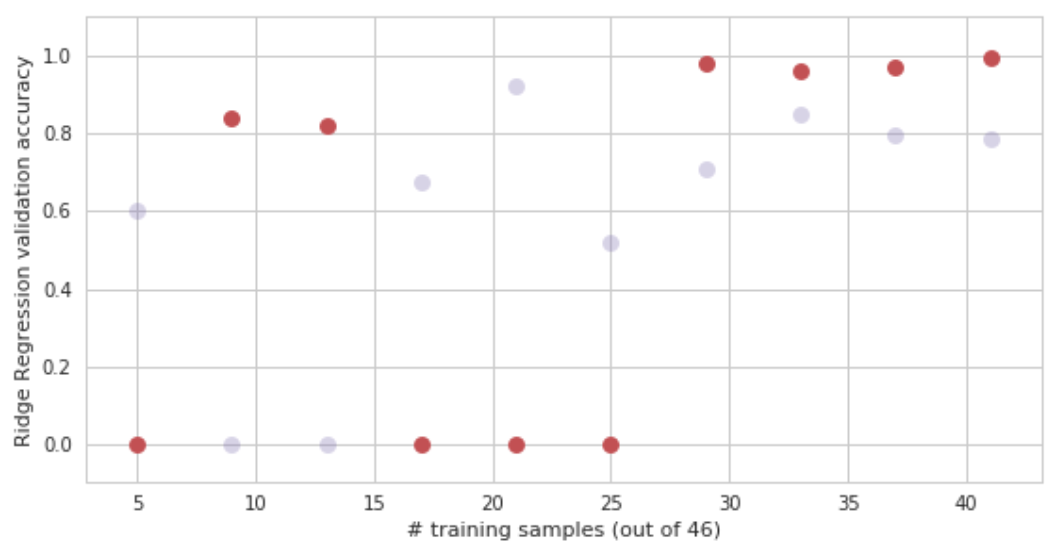
\includegraphics[width=0.5\textwidth]{assets/validation_performance.png}
  \caption{Cross-validation performance on \texttt{Area} prediction via our ridge regression pipeline.}
\end{figure}

\label{Redblue}
\begin{figure}[h!]
	\centering
	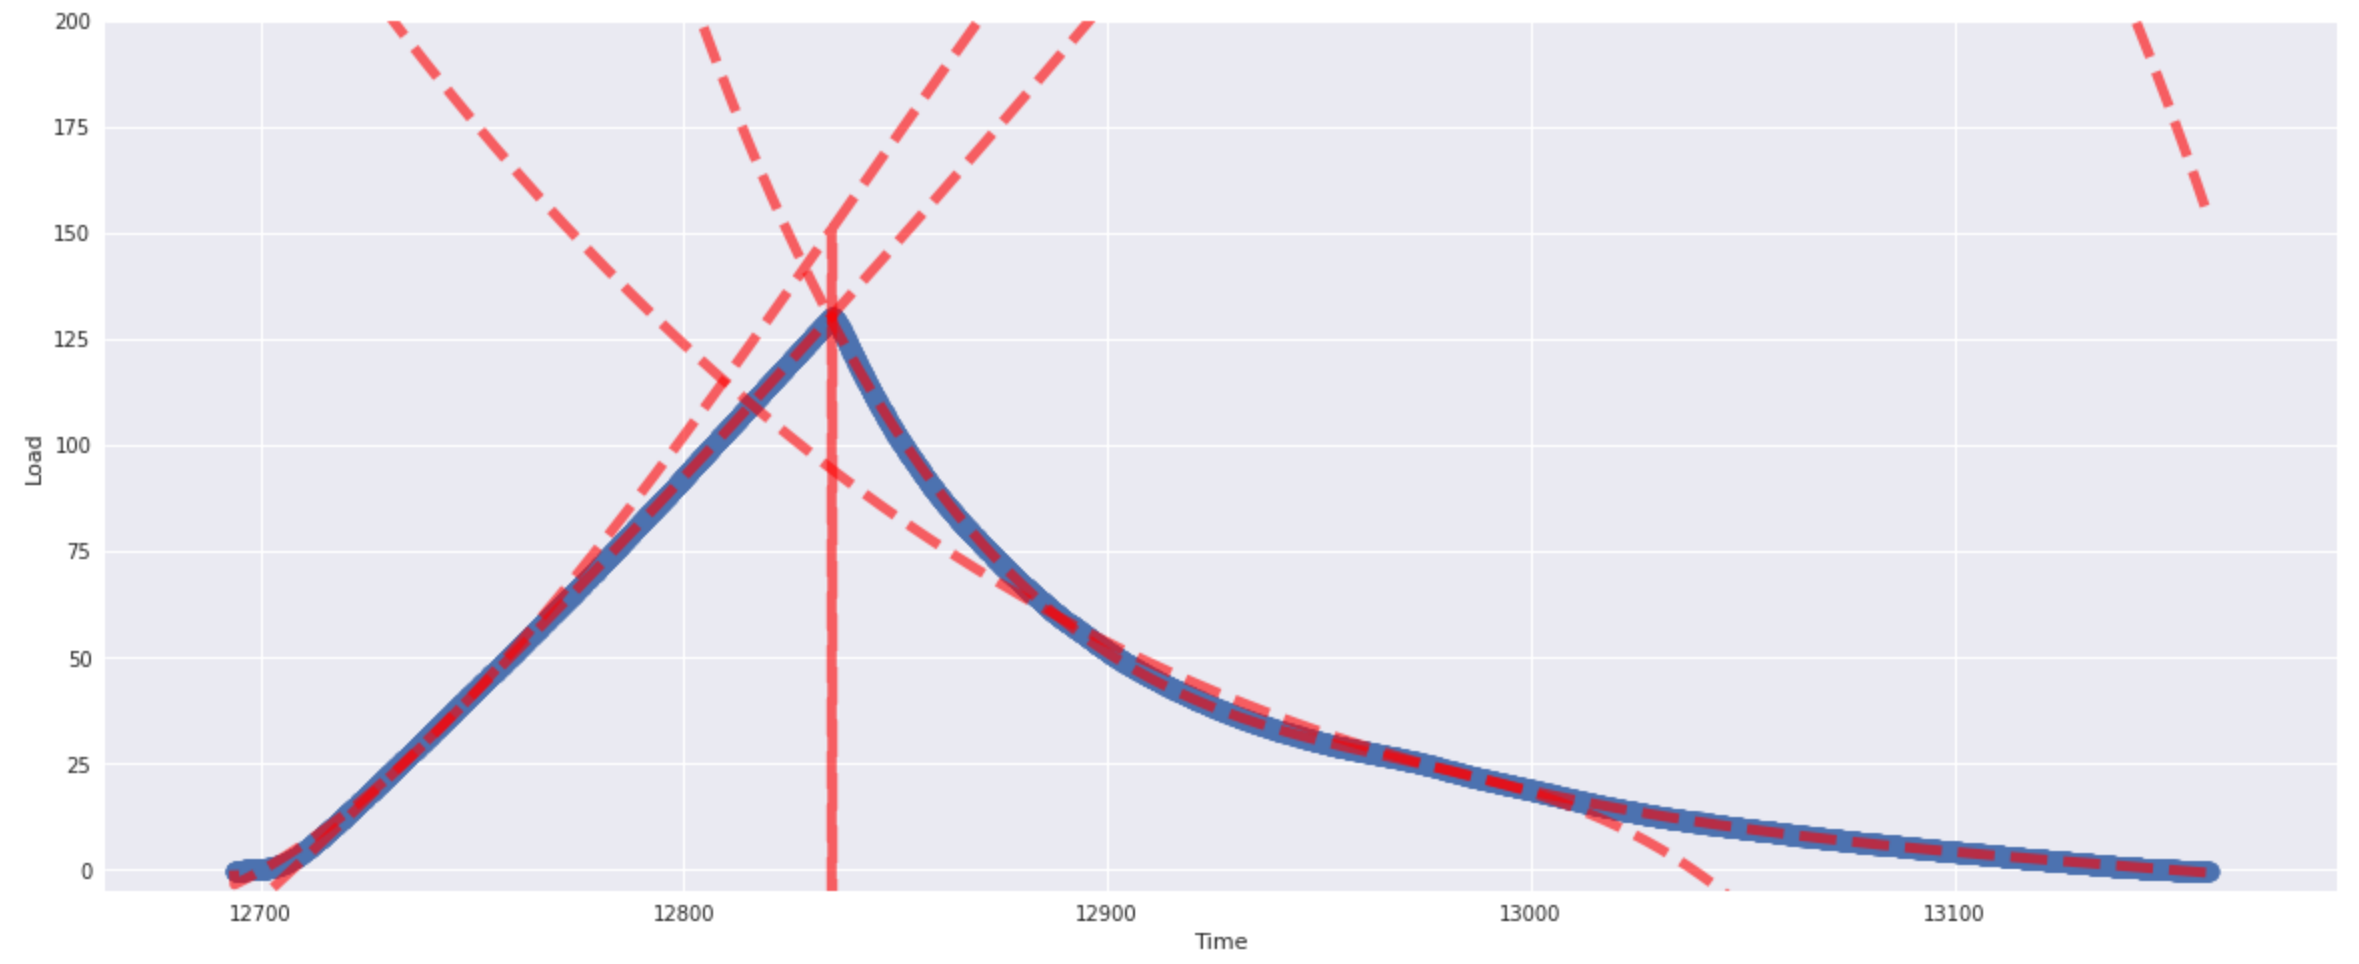
\includegraphics[width=0.5\textwidth]{assets/piecewise_fit.png}
  \caption{Forecasting the $40^{\text{th}}$ cycle \texttt{Load} characteristic, with algorithm trained on $39$ previous cycles. (Predicted piecewise \texttt{Load} curves in \textit{red}; ground truth observations in \textit{blue}).}
\end{figure}

%%%%%%%%%%%%%%%%%%%%%%%%%%%%%%%%% <NN>

\section{Learning Periodic Functions}
We begin by fine-tuning a single model to learn simple periodic functions. As our eventual goal is to predict the behavior of a non-periodic Time series, we opt to similarly treat this task as a Time series forecasting problem in which our samples are not independent, but are rather related to one another across time. Our real data is fairly limited, and so we also attempt to simulate this constraint by only generating 20 cycles for each of the three synthetic datasets.


\subsection{Formatting Data for Supervised Learning}
To build our set of examples, we first calculated the period \textit{P} of a cycle. A single example is formatted such that it contains three full cycles worth of \textit{input} points (\textit{Px3}) and one full cycle worth of \textit{label} points (\textit{P}). We then utilize the "sliding window" method to step along our univariate time series one point at a time, collecting the proceeding \textit{Px4} points to build an example. This process continues along the dataset until there aren't enough remaining points to produce a full \textit{input} and \textit{label} pairing.

The final result is stored in a Pandas Dataframe to be fed into the Neural Network.

\subsection{Network Architecture}
We apply Long short-term memory (LSTM) neural networks to best capture the time dependency of our data. The network's architecture and parameters are depicted in \textbf{Figure 8} and are further summarized below:
\begin{enumerate}
\item Input Layer (\textit{Px3} data points)
\item LSTM Layer  (120 memory gate neurons)
\item Dense Layer (100 neurons)
\item Output Layer (\textit{P} predictions)
\end{enumerate}

\label{PeriodicArchParams}
\begin{figure}[h]
	\centering
	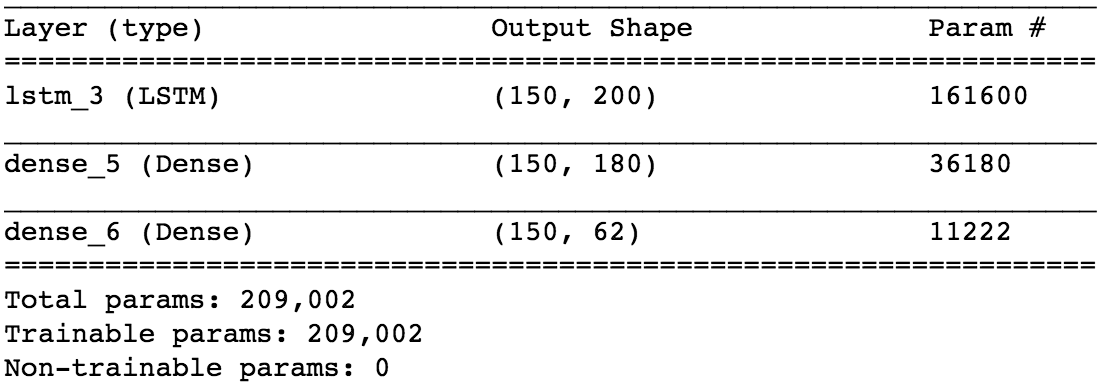
\includegraphics[width=0.5\textwidth]{assets/periodic_arch_params.png}
    \caption{Periodic LSTM architecture parameters.}
\end{figure}




\subsection{Prediction \& Results}
Below are our results on a sine wave, triangle wave, and square wave. Our plots are color coded as follows:

\begin{enumerate}
\item \textbf{Gray}: Training/Validation data
\item \textbf{Blue}: Test example input
\item \textbf{Green}: Test example label
\item \textbf{Red}: Test example forecast
\end{enumerate}

\textit{Note that we can hardly see any green points in the figures-- indicating accurate forecasting results.}

\label{SineForecasting}
\begin{figure}[h]
	\centering
	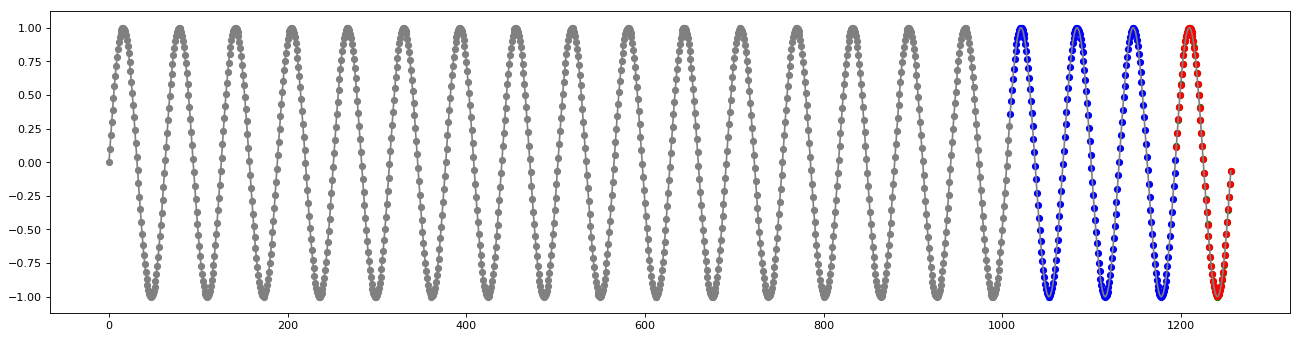
\includegraphics[width=0.5\textwidth]{assets/sine_forecast.png}
    \caption{Forecasting the sine wave with a LSTM network.}
\end{figure}

\label{TriangleForecasting}
\begin{figure}[h]
	\centering
	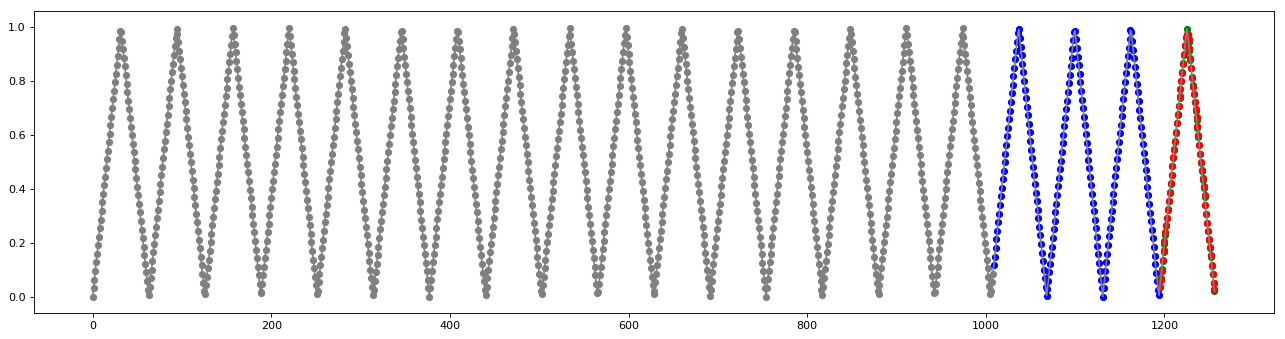
\includegraphics[width=0.5\textwidth]{assets/triangle_forecast.png}
    \caption{Forecasting the Triangle wave with a LSTM network.}
\end{figure}

\label{SquareForecasting}
\begin{figure}[h]
	\centering
	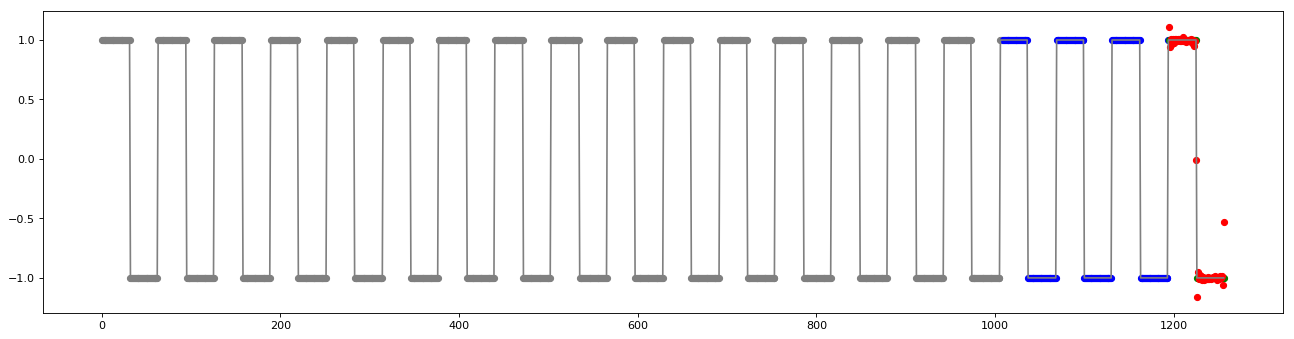
\includegraphics[width=0.5\textwidth]{assets/square_forecast.png}
    \caption{Forecasting the Square wave with a LSTM network.}
\end{figure}

We quantify our prediction results by calculating the \textit{Root Mean Squared Error} (RMSE) and the \textit{Mean Absolute Error} (MAE) percentage for each wave forecast. To calculate the MAE \%, we divide the MAE by the difference between a cycle's peak and trough. In this case, all cycles have the same peak and trough, so we simply subract the \texttt{min} from the \texttt{max} of the data set. By making the error relative to cycle height in order to produce a percentage, our results are more interpretable. 

It appears as though smooth functions are far easier to learn than functions with cusps or discontinuities, as the model was able to achieve the best results on the \texttt{sine} wave with the least training. \textbf{Table IV} contains these results across all three periodic functions, where a \textit{batch size} of 150 examples was used for each. 

It is very interesting to note that the below results were achieved after 1500 epochs for both the square and triangle wave, but only after 100 epochs for the sine wave. It would appear that smooth functions are far easier to learn than ones with cusps or discontinuities. All three waves were trained using a \textit{batch size} of 150 examples.

\label{PeriodicResults}
\begin{table}[h!] % h for here, not the top of the document
  \centering
  \begin{tabular}{ c | c c c }
      Function type & Epochs & MAE \% & RMSE  \\
      \hline
      \verb|Sine| & 100 & 0.111  & 0.003 \\
      \verb|Triangle| & 1500 & 0.439 & 0.005\\
      \verb|Square| & 1500 &1.19 & 0.061

  \end{tabular}
  \caption{Periodic function forecasting results.}
\end{table}

As these results show, using a relative MAE \% metric, we are able to achieve 98+\% accuracy on each of the three curves.

The training plots are provided below, where the validation set is comprised of the last 20\% of the data (excluding the test set). We take the \textit{Mean Squared Error} (MSE) as our error metric. Although we see a very sharp initial error drops and subsequent diminishing returns, 1500 epochs are needed to push past 1\% error on the Triangle wave and 2\% error on the Square wave.  

\begin{figure}[!tbp]
  \centering
  \begin{minipage}[b]{0.4\textwidth}
    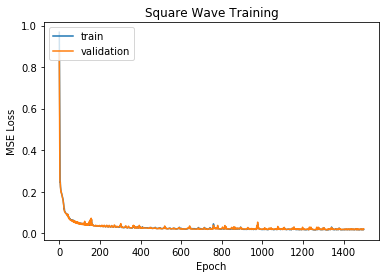
\includegraphics[width=\textwidth]{assets/sine_training_plot.png}
    \caption{Sine training plot.}
  \end{minipage}
  \hfill
  \begin{minipage}[b]{0.4\textwidth}
    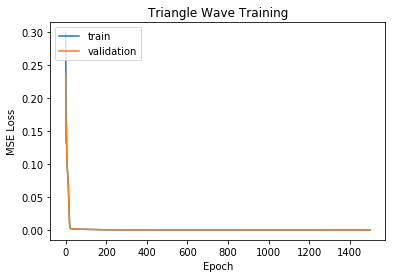
\includegraphics[width=\textwidth]{assets/triangle_training_plot.png}
    \caption{Triangle training plot}
  \end{minipage}
    \begin{minipage}[b]{0.4\textwidth}
    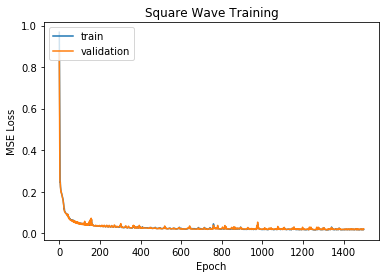
\includegraphics[width=\textwidth]{assets/square_training_plot.png}
    \caption{Square training plot}
  \end{minipage}
\end{figure}







\section{Learning Non-periodic Behavior}

\subsection{Data Formatting}

Our real data is far more dense than our synthetic Sine, Triangle, and Square sets and so we subsample by 60 (take 1 point for every 60) so as to reduce the input dimension to our network. Additionally, the original data formatting phase no longer applies because cycle periods are no longer static and rather require more data points to capture as they grow. We address this by modifying this initial step to handle a variable number of input and output points.

We first perform a  preprocessing step to calculate the period of each cycle based on it's peak and trough locations. We then use the same sliding window method that collects four cycles worth of points for each example. It's important to note that Keras LSTM networks must have a fixed size input and output, and so we store each example in a larger fixed-length array (a \textit{"container"}). This length is preset and is always larger than an example worth of points, so as to not loose information. We represent \textit{Null} values with -10. To help ensure that the network doesn't confuse these values with real data, we shift all data points until the smallest value is 0.

Upon the completion of this step, we have a Pandas data frame that effectively holds variable-length examples.

\subsection{Network Architecture}

Just as before, we use LSTM layer's to capture the time dependent nature of our data. However, we increase the complexity of our model as it now needs to learn substantially more complex behavior, including period growth and distortions to the curve's belly and back. We now apply two consecutive LSTM layers rather than one to create a more complex hierarchical feature representation of the input data. This is then feed into a dense hidden layer to extract one last feature vector to be fed into the output. The network's architecture and parameters are shown in \textbf{Figure 15} and are further summarized below:

\begin{enumerate}
\item Input Layer (\textit{Px3} data points)
\item LSTM Layer  (400 memory gate neurons)
\item LSTM Layer  (256 memory gate neurons)
\item Dense Layer (128 neurons)
\item Output Layer (\textit{P} predictions)
\end{enumerate}

\label{NonperiodicParams}
\begin{figure}[!h]
	\centering
	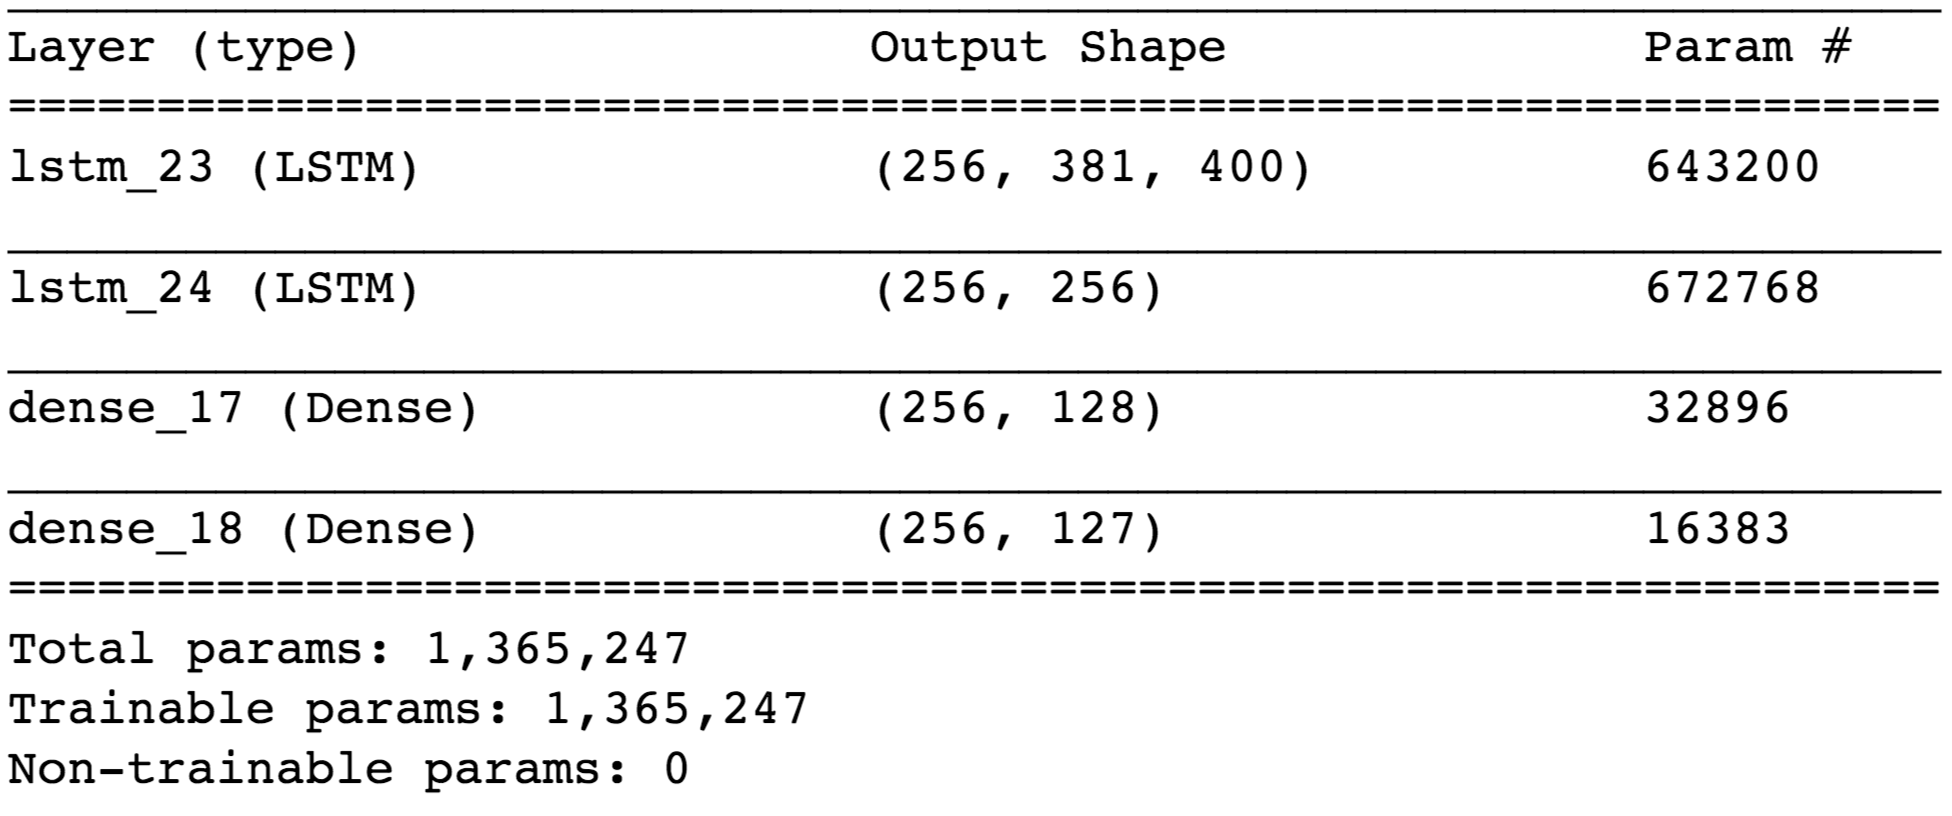
\includegraphics[width=0.5\textwidth]{assets/non_periodic_params.png}
    \caption{Non-periodic LSTM architecture parameters.}
\end{figure}

Keras LSTM layers take in input and produce output in the form:(\texttt{batch\_size}, \texttt{timesteps}, \texttt{input\_dimension}) where \texttt{batch\_size} is 256, \texttt{timesteps} is Px3, and \texttt{input\_dimension} is 1 as our time series is of one variable.





\subsection{Prediction \& Results}

In \textbf{Figure 16}, \textbf{Figure 17}, and \textbf{Figure 18}} we show the entire training and test set (47 cycles) split into thirds stacked on top of one another to best contrast the growth of each period over time. 
Just as before, we color code the plots as follows:
\begin{enumerate}
\item \textbf{Gray}: Training/Validation data
\item \textbf{Blue}: Test example input
\item \textbf{Green}: Test example label
\item \textbf{Red}: Test example forecast
\end{enumerate}

\label{LoadTimeForecasts1}
\begin{figure}[!h]
	\centering
	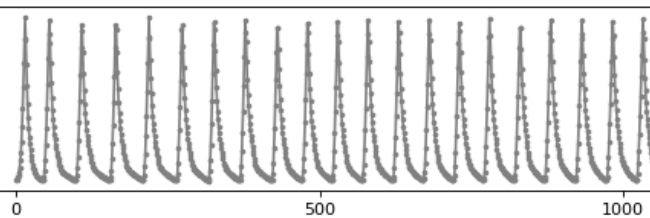
\includegraphics[width=0.5\textwidth]{assets/loadtime_prediction_slice1.png}
    \caption{First third of data set.}
\end{figure}

\label{LoadTimeForecasts2}
\begin{figure}[!h]
	\centering
	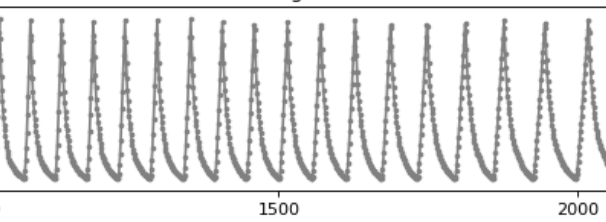
\includegraphics[width=0.5\textwidth]{assets/loadtime_prediction_slice2.png}
    \caption{Second third of data set.}
\end{figure}

\label{LoadTimeForecasts3}
\begin{figure}[!h]
	\centering
	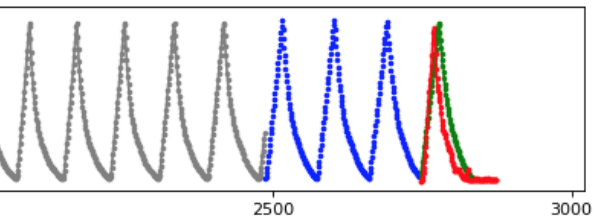
\includegraphics[width=0.5\textwidth]{assets/loadtime_prediction_slice3.png}
    \caption{Last part of data set and forecasts.}
\end{figure}


In \textbf{Figure 19} we plot the \textit{MSE} network loss over epochs of training. It is clear that the network is appropriately tuned to avoid both under-fitting and over-fitting, as the training loss and validation loss are in near lock-step with one another.

\label{LoadTimeTraining}
\begin{figure}[!h]
	\centering
	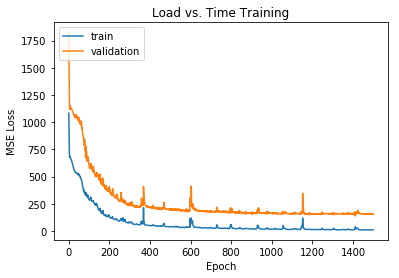
\includegraphics[width=0.5\textwidth]{assets/loadtime_training_plot.png}
    \caption{Load vs. Time loss plot.}
\end{figure}


Our best results running this experiment resulted in a Mean Absolute Error (MAE) percentage of \textit{16.25}, and a Root Mean Square Error (RMSE) loss of \textit{25.3}, and a predicted period of \textit{72} while the true period was \textit{88}. This still implies that the network learned to factor in period growth, as the initial training examples contained periods as low as \textit{54}.

%%%%%%%%%%%%%%%%%%%%%%%%%%%%%%%% </NN>


\section{Miscellaneous approaches}
\subsection{Fourier analysis}
Fourier analysis on cycle \verb|Load| and \verb|Time| behavior may reveal oscillatory components underlying the complex actuator \verb|Load| characteristic. Applying a discrete Fourier transform (DFT) to raw cycle data results in a DFT magnitude response with some easily-identifiable important frequencies, as seen in \textbf{Figure 20}.

While some frequencies clearly have stronger DFT magnitude than others, Fourier analysis does not effectively capture the varying \verb|Period| phenomena that drives the \verb|Load| characteristic of the actuator. Extrapolating the top-$1000$ frequencies from DFT analysis enables the $48^{\text{th}}$-cycle prediction shown in \textbf{Figure 21}.

\label{Logfourier}
\begin{figure}[h!]
	\centering
	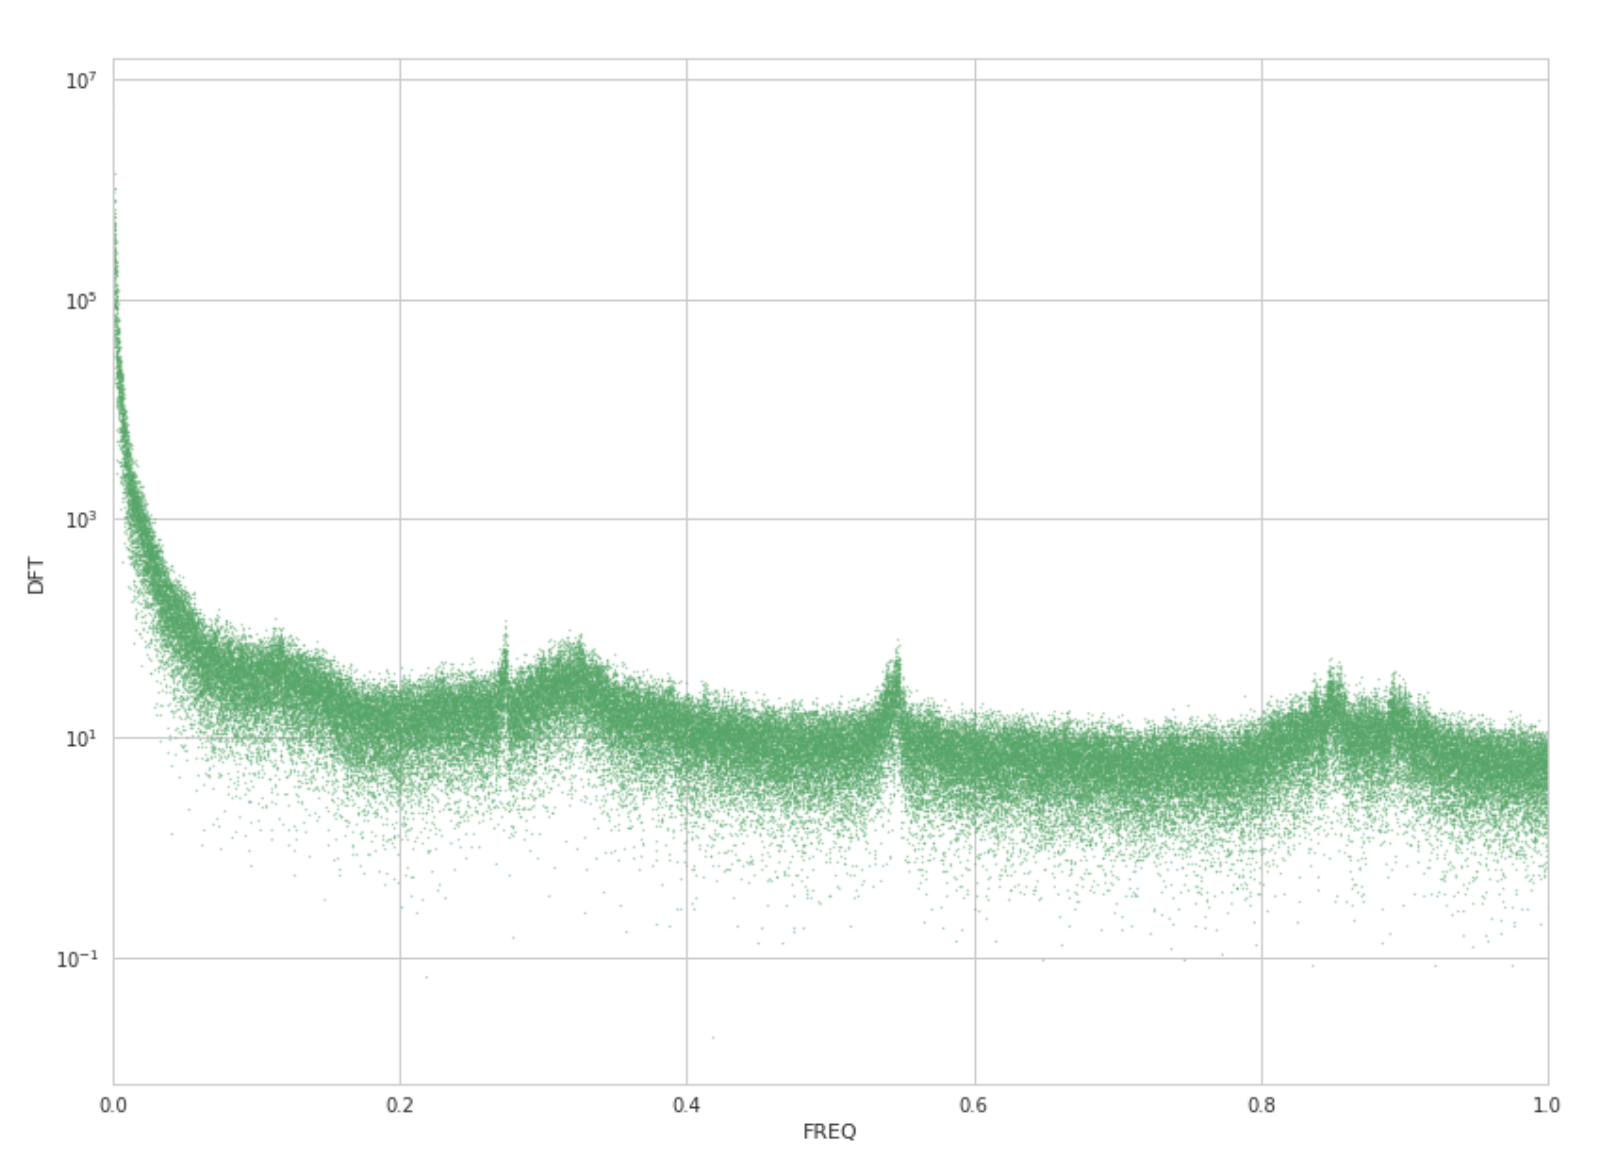
\includegraphics[width=0.5\textwidth]{assets/fourier_analysis.png}
  \caption{Discrete Fourier transform (log-magnitude) of raw cycle data.}
\end{figure}

\label{Extrapolation}
\begin{figure}[h!]
	\centering
	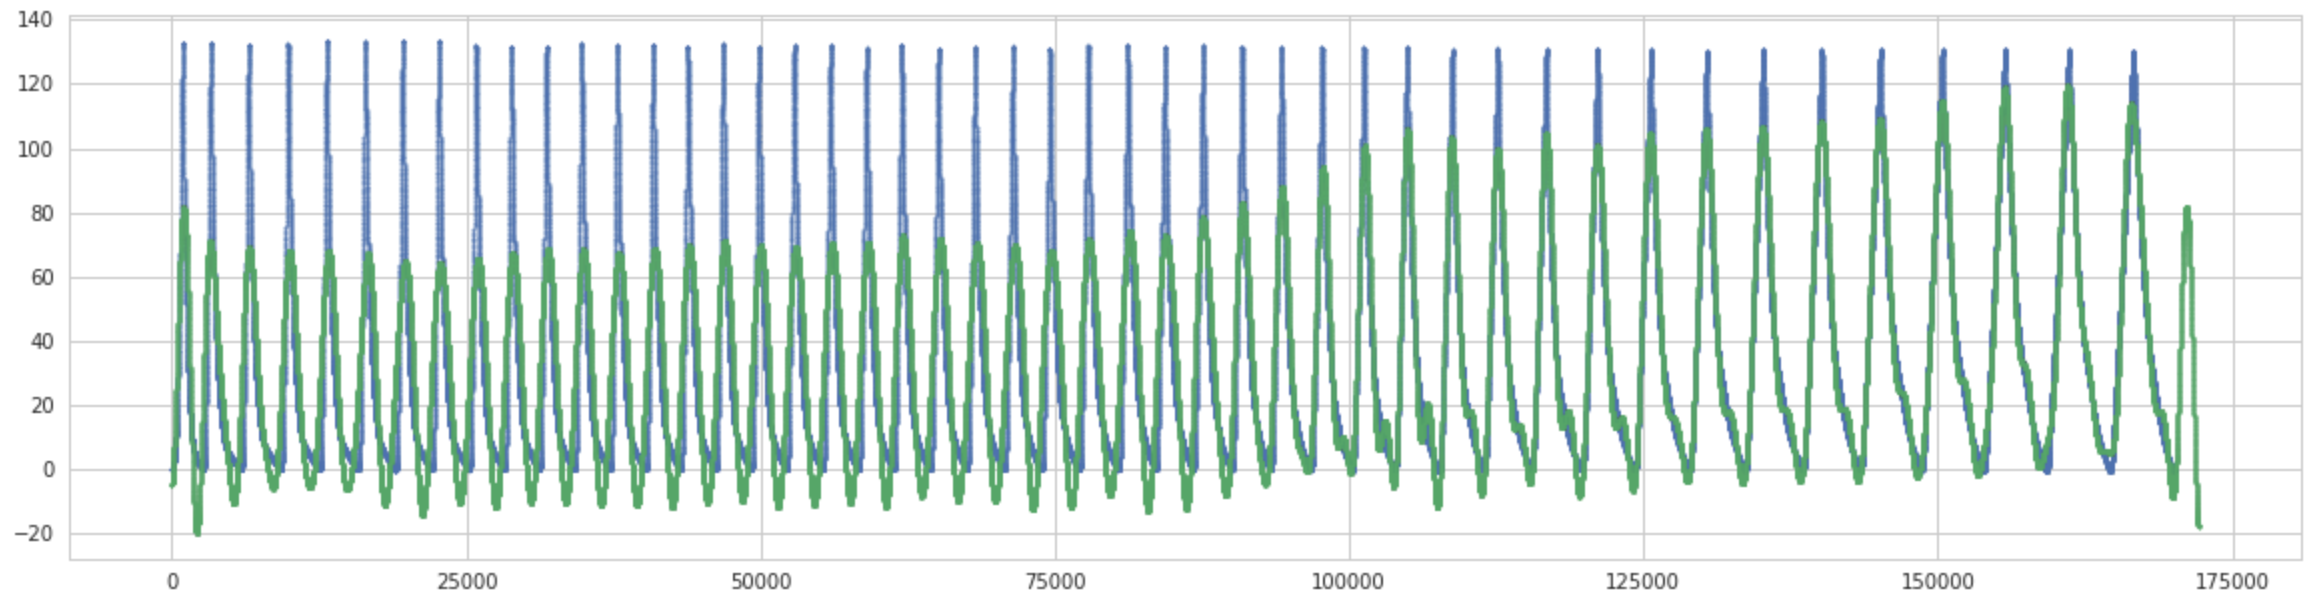
\includegraphics[width=0.5\textwidth]{assets/fourier_extrapolation.png}
  \caption{Extrapolation of top-$1000$ frequencies from DFT analysis. Ground truth in \textit{blue}; prediction in \textit{green}.}
\end{figure}

\subsection{Time-series analysis}

Conventional time-series methods, including autoregressive integrated moving average (ARIMA) models tuned to take into account non-linear trends and non-constant periodicity, were attempted. These models performed poorly, but parts of our methodology in using them are included here for the benefit of future work.

\textbf{Figure 22} depicts the autocorrelation behavior of the raw cycle signal, where \textit{Lag} measures delay in units of cycle index. We observe little correlation between delayed windows of cycles, varying inversely with lag.

\label{Autocorrelation}
\begin{figure}[h]
	\centering
	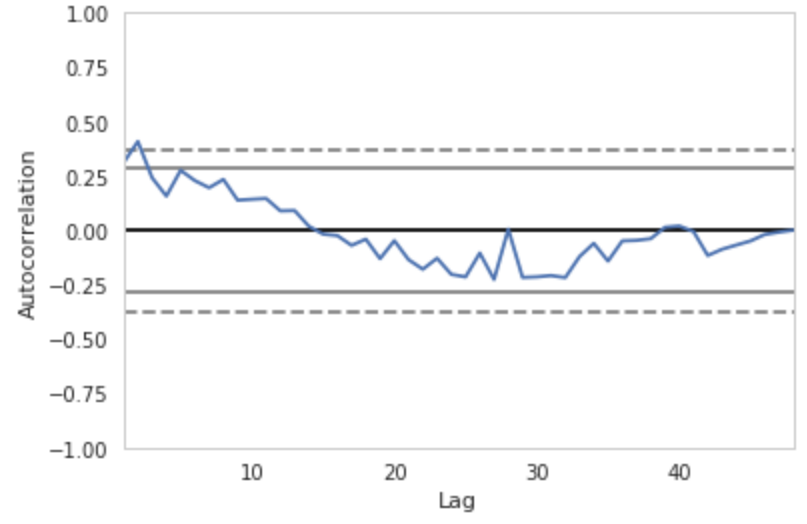
\includegraphics[width=0.45\textwidth]{assets/autocorrelation.png}
  \caption{(Serial) autocorrelation of cycles. Horizontal lines correspond to $95\%$ and $99\%$ confidence bands.}
\end{figure}

\section{FUTURE WORK}
Miriyev et al.$^1$ describe a closed-form approach to approximating the diffusion behavior of this actuator system. Future work may more accurately model the heating/cooling \verb|Load| characteristic of the actuator using this additional feature.

\section*{ACKNOWLEDGMENT}

We would like to acknowledge \href{http://aslanmiriyev.com/}{Aslan Miriyev (Ph.D.)} and \href{https://www.hodlipson.com/}{Professor Hod Lipson} for their vision and expert mentorship over the course of this work, and for the providing the opportunity to work with unique and powerful data and hardware. We also thank \href{http://ogchang.com/}{Oscar Chang}, \href{http://www.cs.columbia.edu/~bchen/}{Boyuan Chen}, and \href{http://www.cs.columbia.edu/~dechant/}{Chad DeChant} at the \href{https://www.creativemachineslab.com/}{Creative Machines Lab}, administered by Professor Lipson, for their patient and insightful guidance.

\begin{thebibliography}{99}

\bibitem{c1} Miriyev, A., Trujillo, C., Caires, G., & Lipson, H. (2018). Rejuvenation of soft material–actuator. MRS Communications, 1-6. doi:10.1557/mrc.2018.30

\end{thebibliography}

\end{document}
